\documentclass{standalone}
\usepackage{tikz}
\usepackage{ctex,siunitx,ninecolors}
\setCJKmainfont{Noto Serif CJK SC}
\usepackage{tkz-euclide}
\usepackage{amsmath}
\usepackage{wasysym}
\usetikzlibrary{patterns, calc}
\usetikzlibrary{decorations.pathmorphing, decorations.pathreplacing, decorations.shapes,3d}
\begin{document}
\small
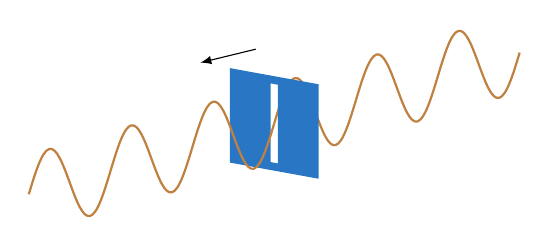
\begin{tikzpicture}[>=latex,z={(30:3mm)},x={(-20:5mm)},yscale=0.5]
  \def\wave{
  \draw[thick,brown]
  (0,0) sin (1,1) cos (2,0) sin (3,-1) cos (4,0)
  sin (5,1) cos (6,0) sin (7,-1) cos (8,0)
  sin (9,1) cos (10,0)sin (11,-1)cos (12,0);
  }
  \begin{scope}[canvas is zy plane at x=0]
  \wave
  \end{scope}
  \begin{scope}[canvas is xy plane at z=0]
    \fill[azure5,even odd rule](-1.2,1.2)rectangle(1.2,-1.2)(-0.1,1.0)rectangle(0.1,-1.0);
  \end{scope}
  \begin{scope}[canvas is zy plane at x=0]
    \begin{scope}[xshift=-12cm]
      \wave
    \end{scope}
    \end{scope}
    \draw [->] (-0.5,1.8)--(-2,1.2);
  \end{tikzpicture}
\end{document}